\section{Resultados del amplificador de potencia} \label{sec:resultados_pa}
El amplificador de potencia fue caracterizado experimentalmente abarcando su comportamiento de pequeña señal, su desempeño de potencia en gran señal y su comportamiento no lineal. A continuación se presentan dichos resultados, junto con la comparación frente a los valores obtenidos mediante simulación en ADS.

% -----------------------------------------------------------------------------------------------%
\subsection{Parámetros dispersión medidos}
Los parámetros dispersión fueron medidos utilizando la configuración de medición descripta en la Figura~\ref{fig:setup_medicion_sparam_amp}, cuya implementación real en el laboratorio de la CNEA se observa en la Figura~\ref{fig:setup_cnea_sparams}.

\begin{figure}[H]
    \centering
    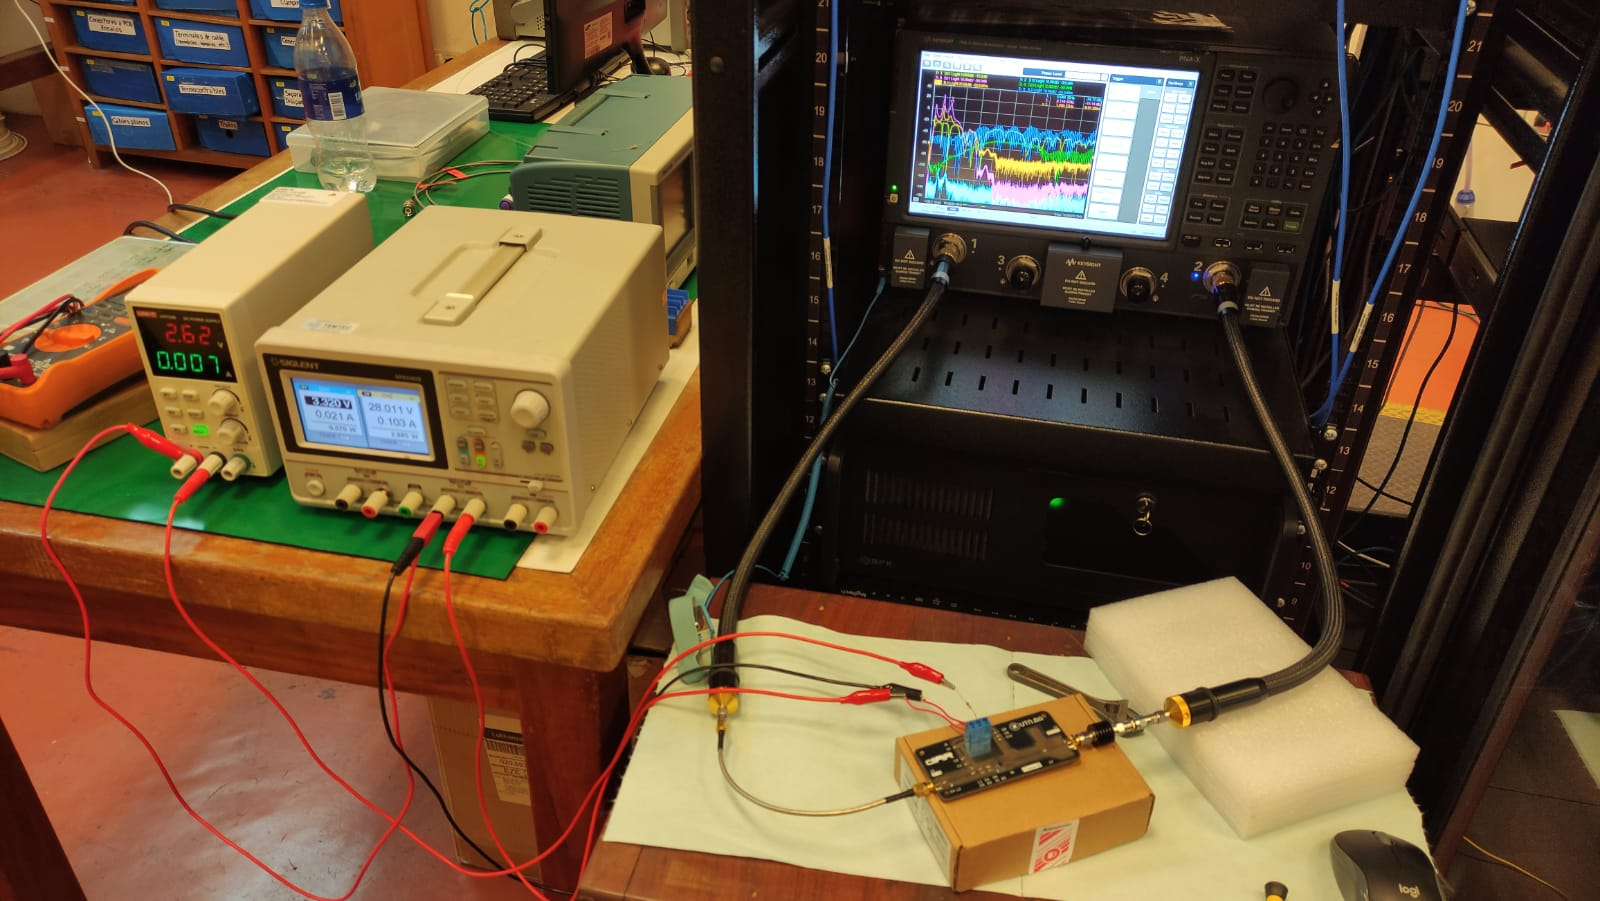
\includegraphics[width=\linewidth]{Figures/08/pa_setup_sparams.jpg}
    \caption{Configuración de instrumentos utilizada para la medición de parámetros dispersión del amplificador de potencia en la CNEA.}
    \label{fig:setup_cnea_sparams}
\end{figure}

Las Figuras~\ref{fig:s11_meas} y \ref{fig:s21_meas} presentan los parámetros $S_{11}$ y $S_{21}$ simulados y medidos, respectivamente, en el rango de frecuencias de DC a 5\,GHz. En la respuesta medida se identificó una resonancia fuera de la banda de interés cercana a 1,2~\,GHz indicada en naranja en ambas figuras. Esta característica no fue predicha por el modelo de simulación original y se atribuye a efectos parásitos del layout de la placa y del empaquetado de los componentes que no fueron completamente capturados en el modelo inicial.

\begin{figure}[H]
    \centering
    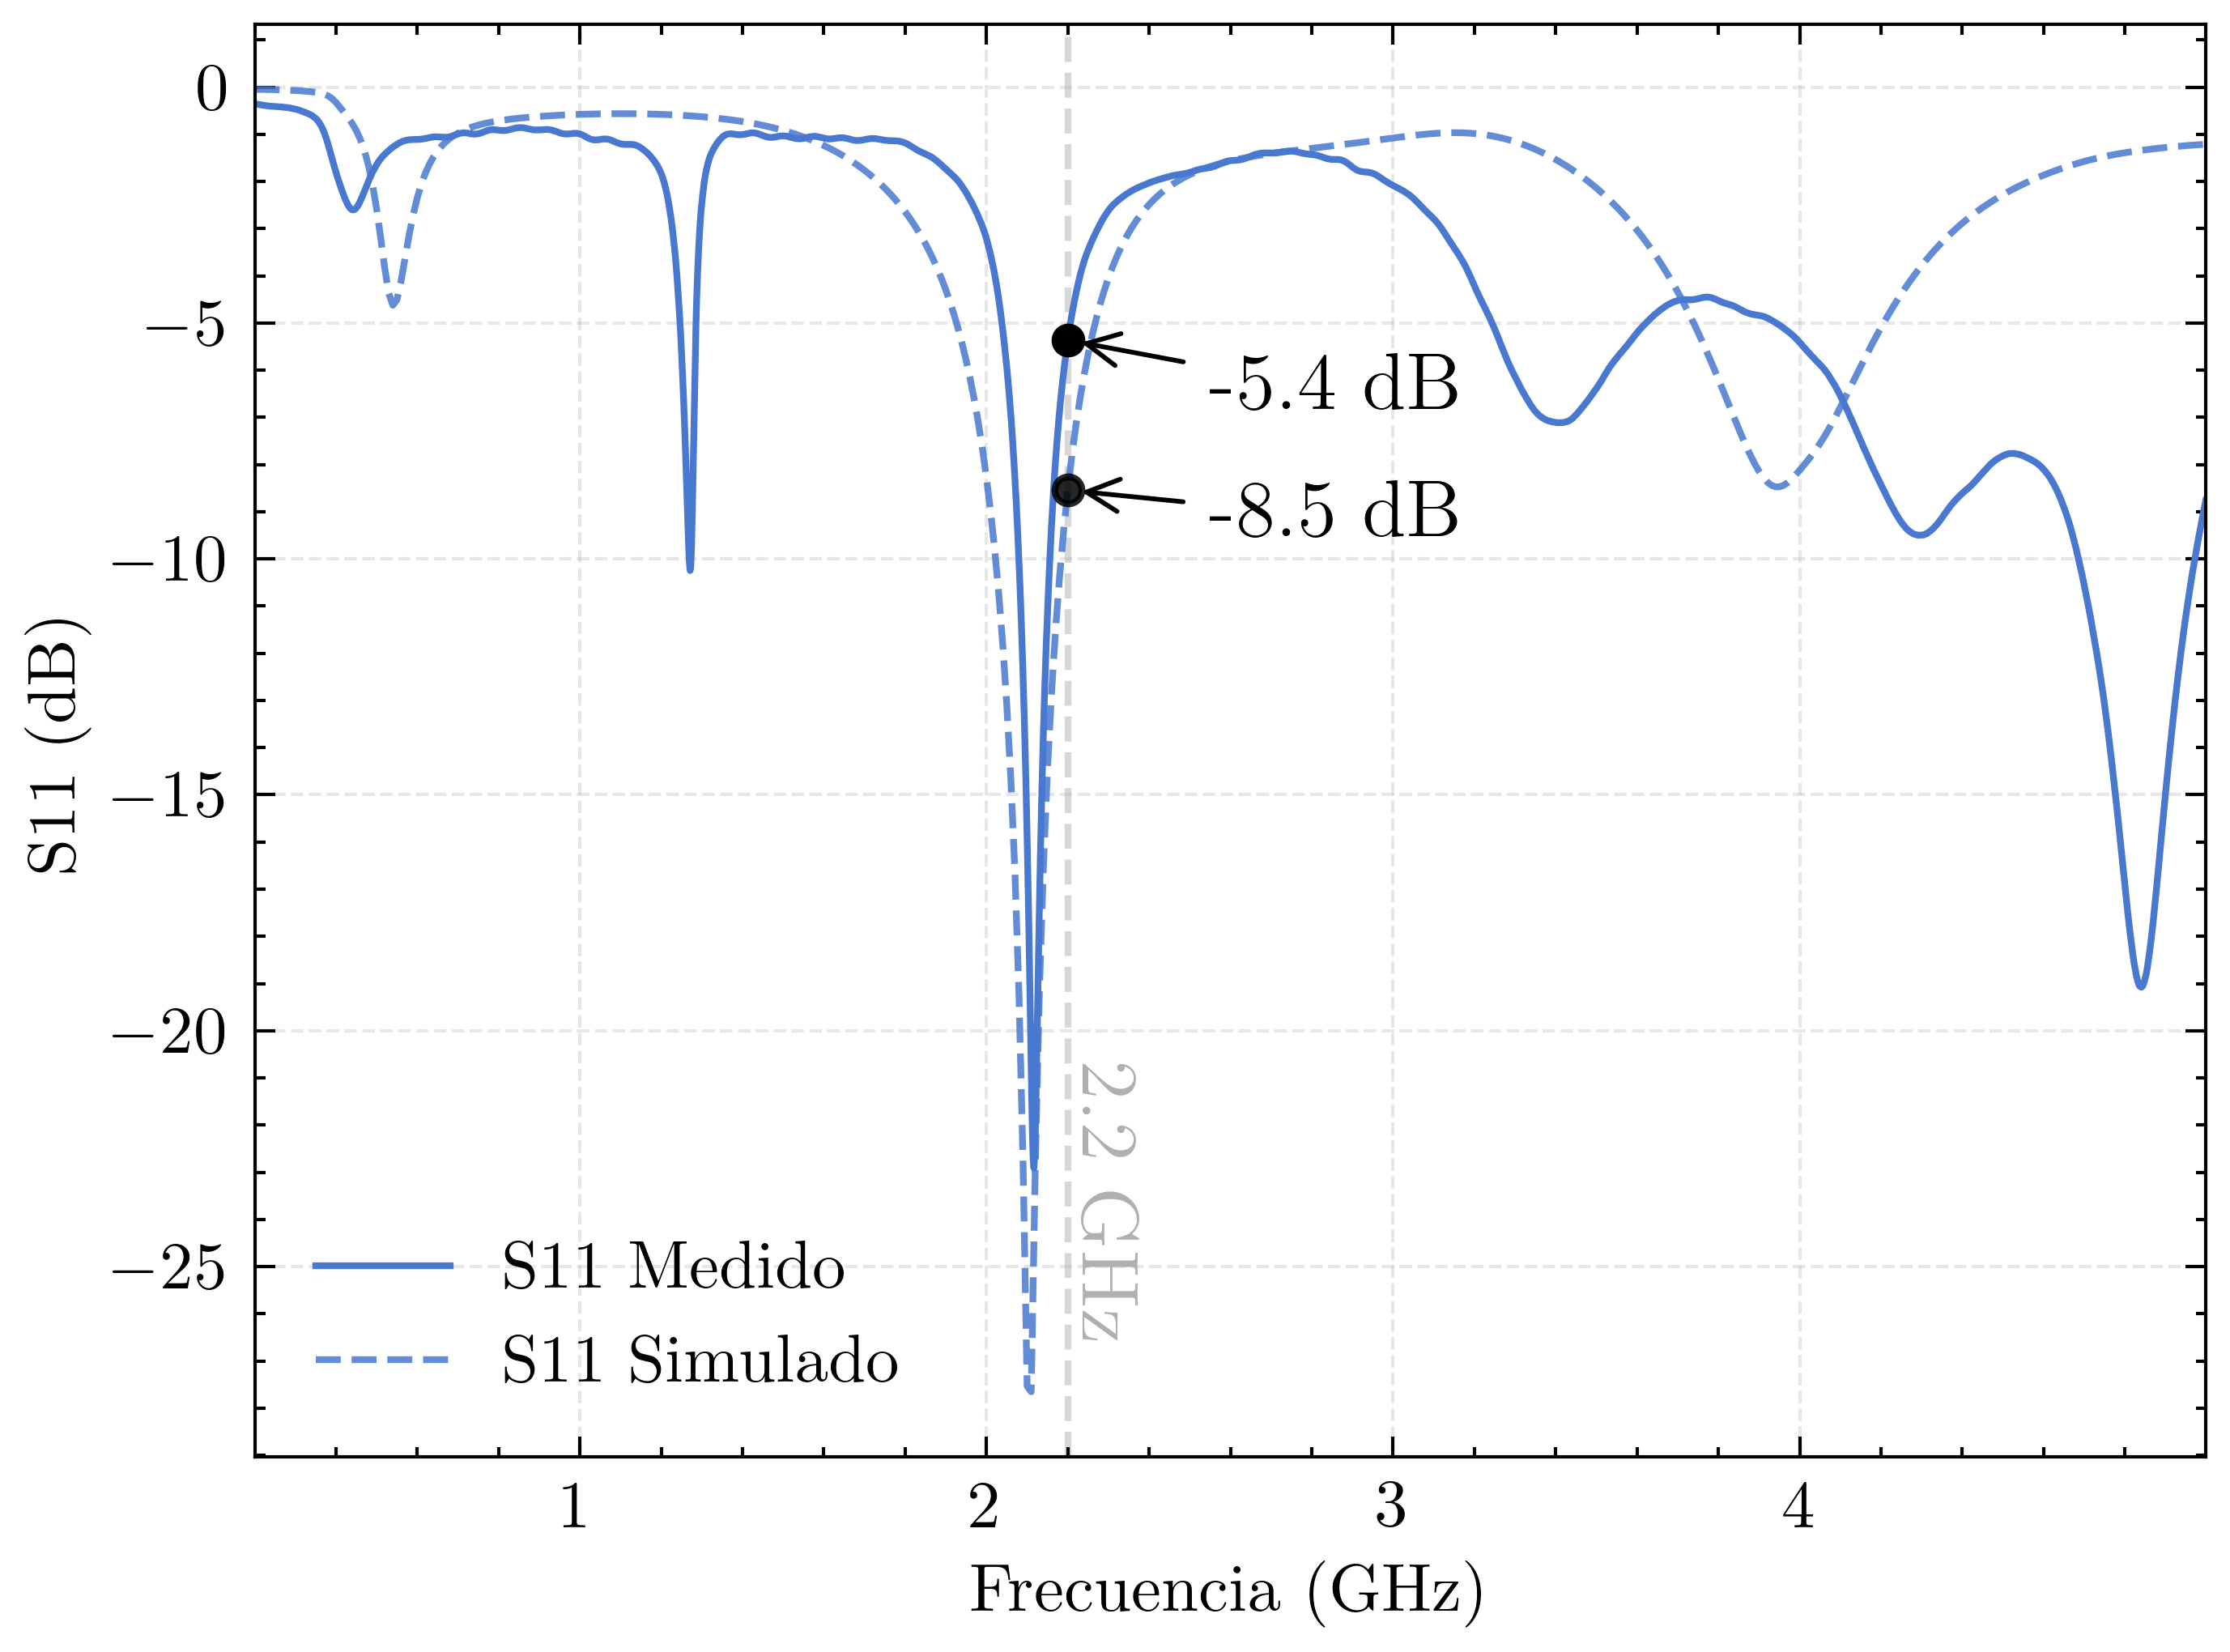
\includegraphics[width=0.7\linewidth]{Figures/08/pa_s11_meas.png}
    \caption{Comparación entre el $S_{11}$ simulado (línea punteada) y medido (línea sólida) del amplificador de potencia fabricado con la resonancia no predicha indicada en naranja.}
    \label{fig:s11_meas}
\end{figure}

\begin{figure}[H]
    \centering
    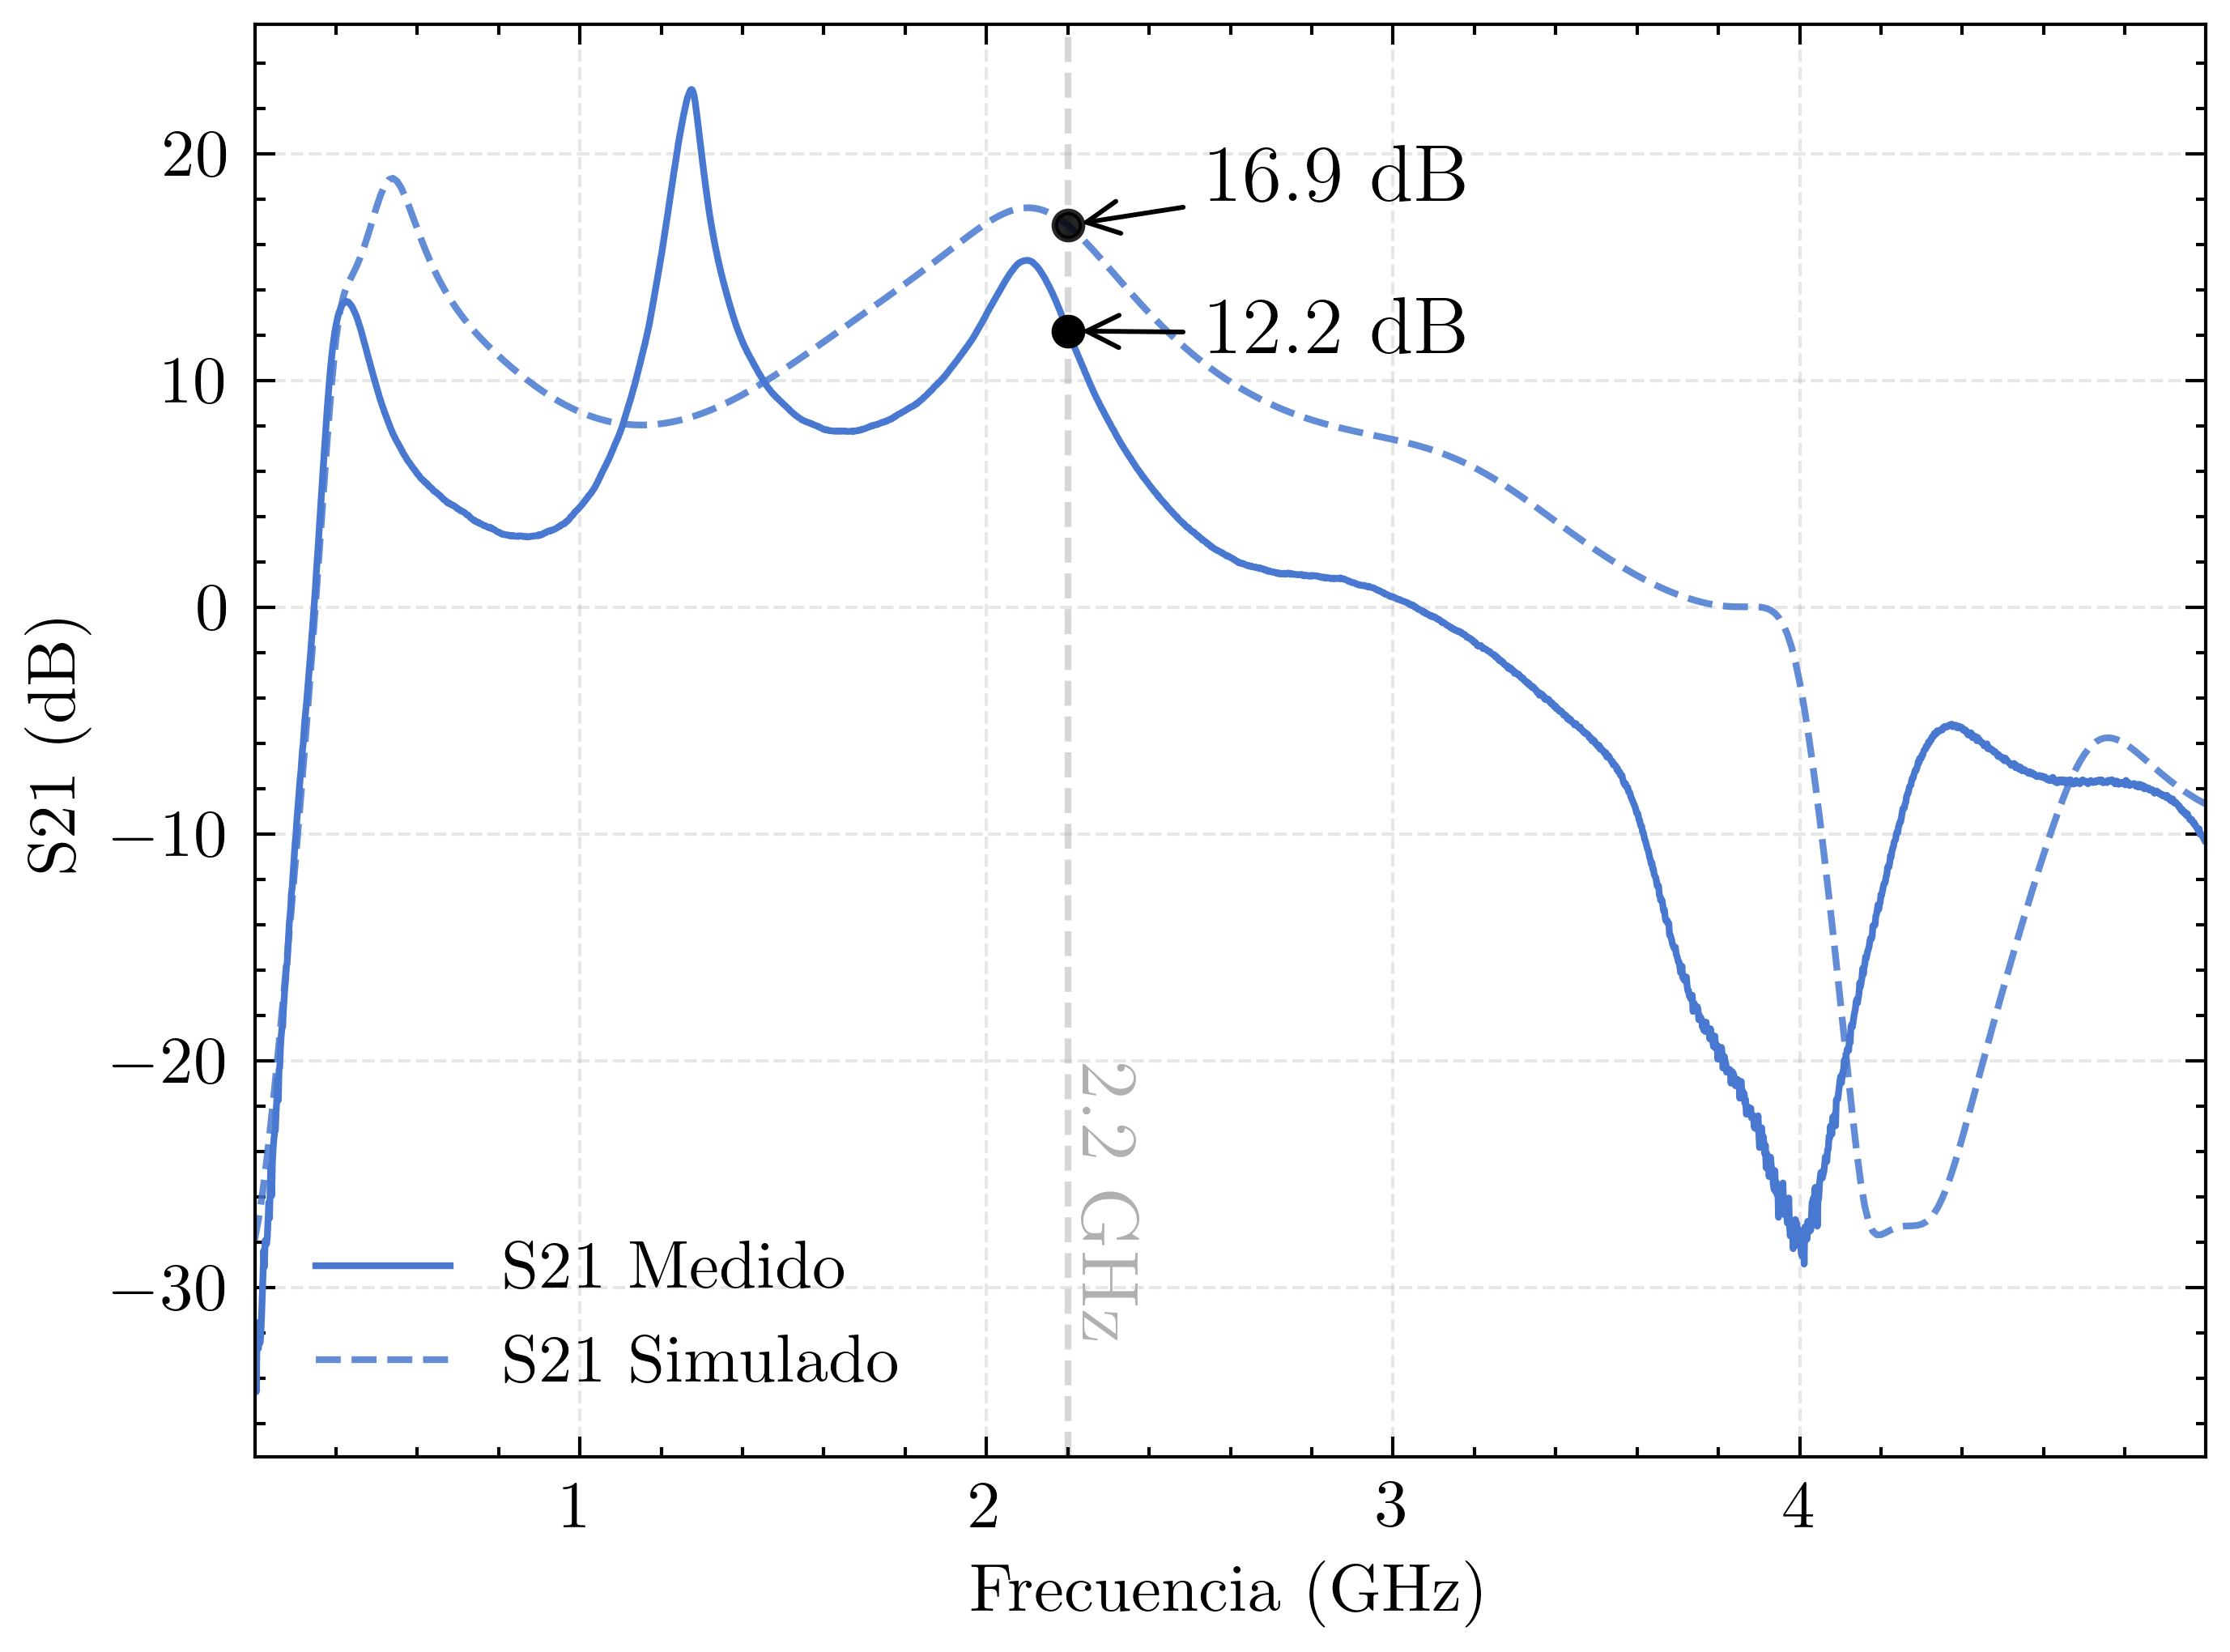
\includegraphics[width=0.7\linewidth]{Figures/08/pa_s21_meas.png}
    \caption{Comparación entre el $S_{21}$ simulado (línea punteada) y medido (línea sólida) del amplificador de potencia fabricado con la resonancia no predicha indicada en naranja.}
    \label{fig:s21_meas}
\end{figure}

En la frecuencia de operación de 2,2\,GHz, el $S_{11}$ medido alcanza -5,4\,dB frente a un valor simulado de -8,5\,dB, mientras que el $S_{21}$ medido en dicho punto es de 12,2\,dB frente a los 16,9\,dB previstos por la simulación. Esta discrepancia resulta consistente con el corrimiento de la frecuencia central descripto a continuación, dado que ambos parámetros se evalúan en un punto de la banda que ya no coincide exactamente con el mínimo de reflexión ni con el máximo de ganancia efectivamente alcanzados por el circuito fabricado.

La frecuencia central medida es de 2,11\,GHz, lo que corresponde a un desplazamiento de 90\,MHz respecto del objetivo de diseño. Este desplazamiento se atribuye a la inductancia equivalente serie (ESL) de las resistencias de la red de estabilidad, correspondiente a los inductores L7 y L8 incorporados en serie con las resistencias R5 y R3 en el esquemático de la Figura~\ref{fig:pa_ads_final}. Al incorporar estas ESL de 0,5\,nH por resistencia, valor consistente con datos publicados para resistencias de película fina en encapsulado 0603~\cite{VishayTN}, la frecuencia central simulada queda en concordancia con la medición, como ilustra la figura. El comportamiento general de pequeña señal resulta consistente con la intención de diseño.

\subsection{Extracción del P1dB}
La Figura~\ref{fig:p1db} muestra la potencia de salida y la ganancia, medidas con el setup de la Figura~\ref{fig:setup_cnea_pout}, en función de la potencia de entrada para la cadena compuesta por el amplificador driver y el amplificador bajo prueba. Dado que el amplificador driver ingresa en compresión dentro del rango de medición, el P1dB del dispositivo bajo prueba no puede leerse directamente de la curva de potencia de salida medida. Por este motivo, se aplicó la expresión de compresión en cascada de la ecuación~\eqref{eq:p1db_cascada}, que refiere la compresión de cada etapa a la entrada del sistema y combina sus contribuciones ponderadas inversamente por la ganancia de las etapas precedentes. El P1dB del amplificador bajo prueba se extrajo resolviendo esta expresión a partir de la ganancia y los valores de compresión conocidos de la etapa driver, obteniéndose un P1dB de 30,3\,dBm (1,07\,W) a una frecuencia de 2,2\,GHz.

\begin{figure}[H]
    \centering
    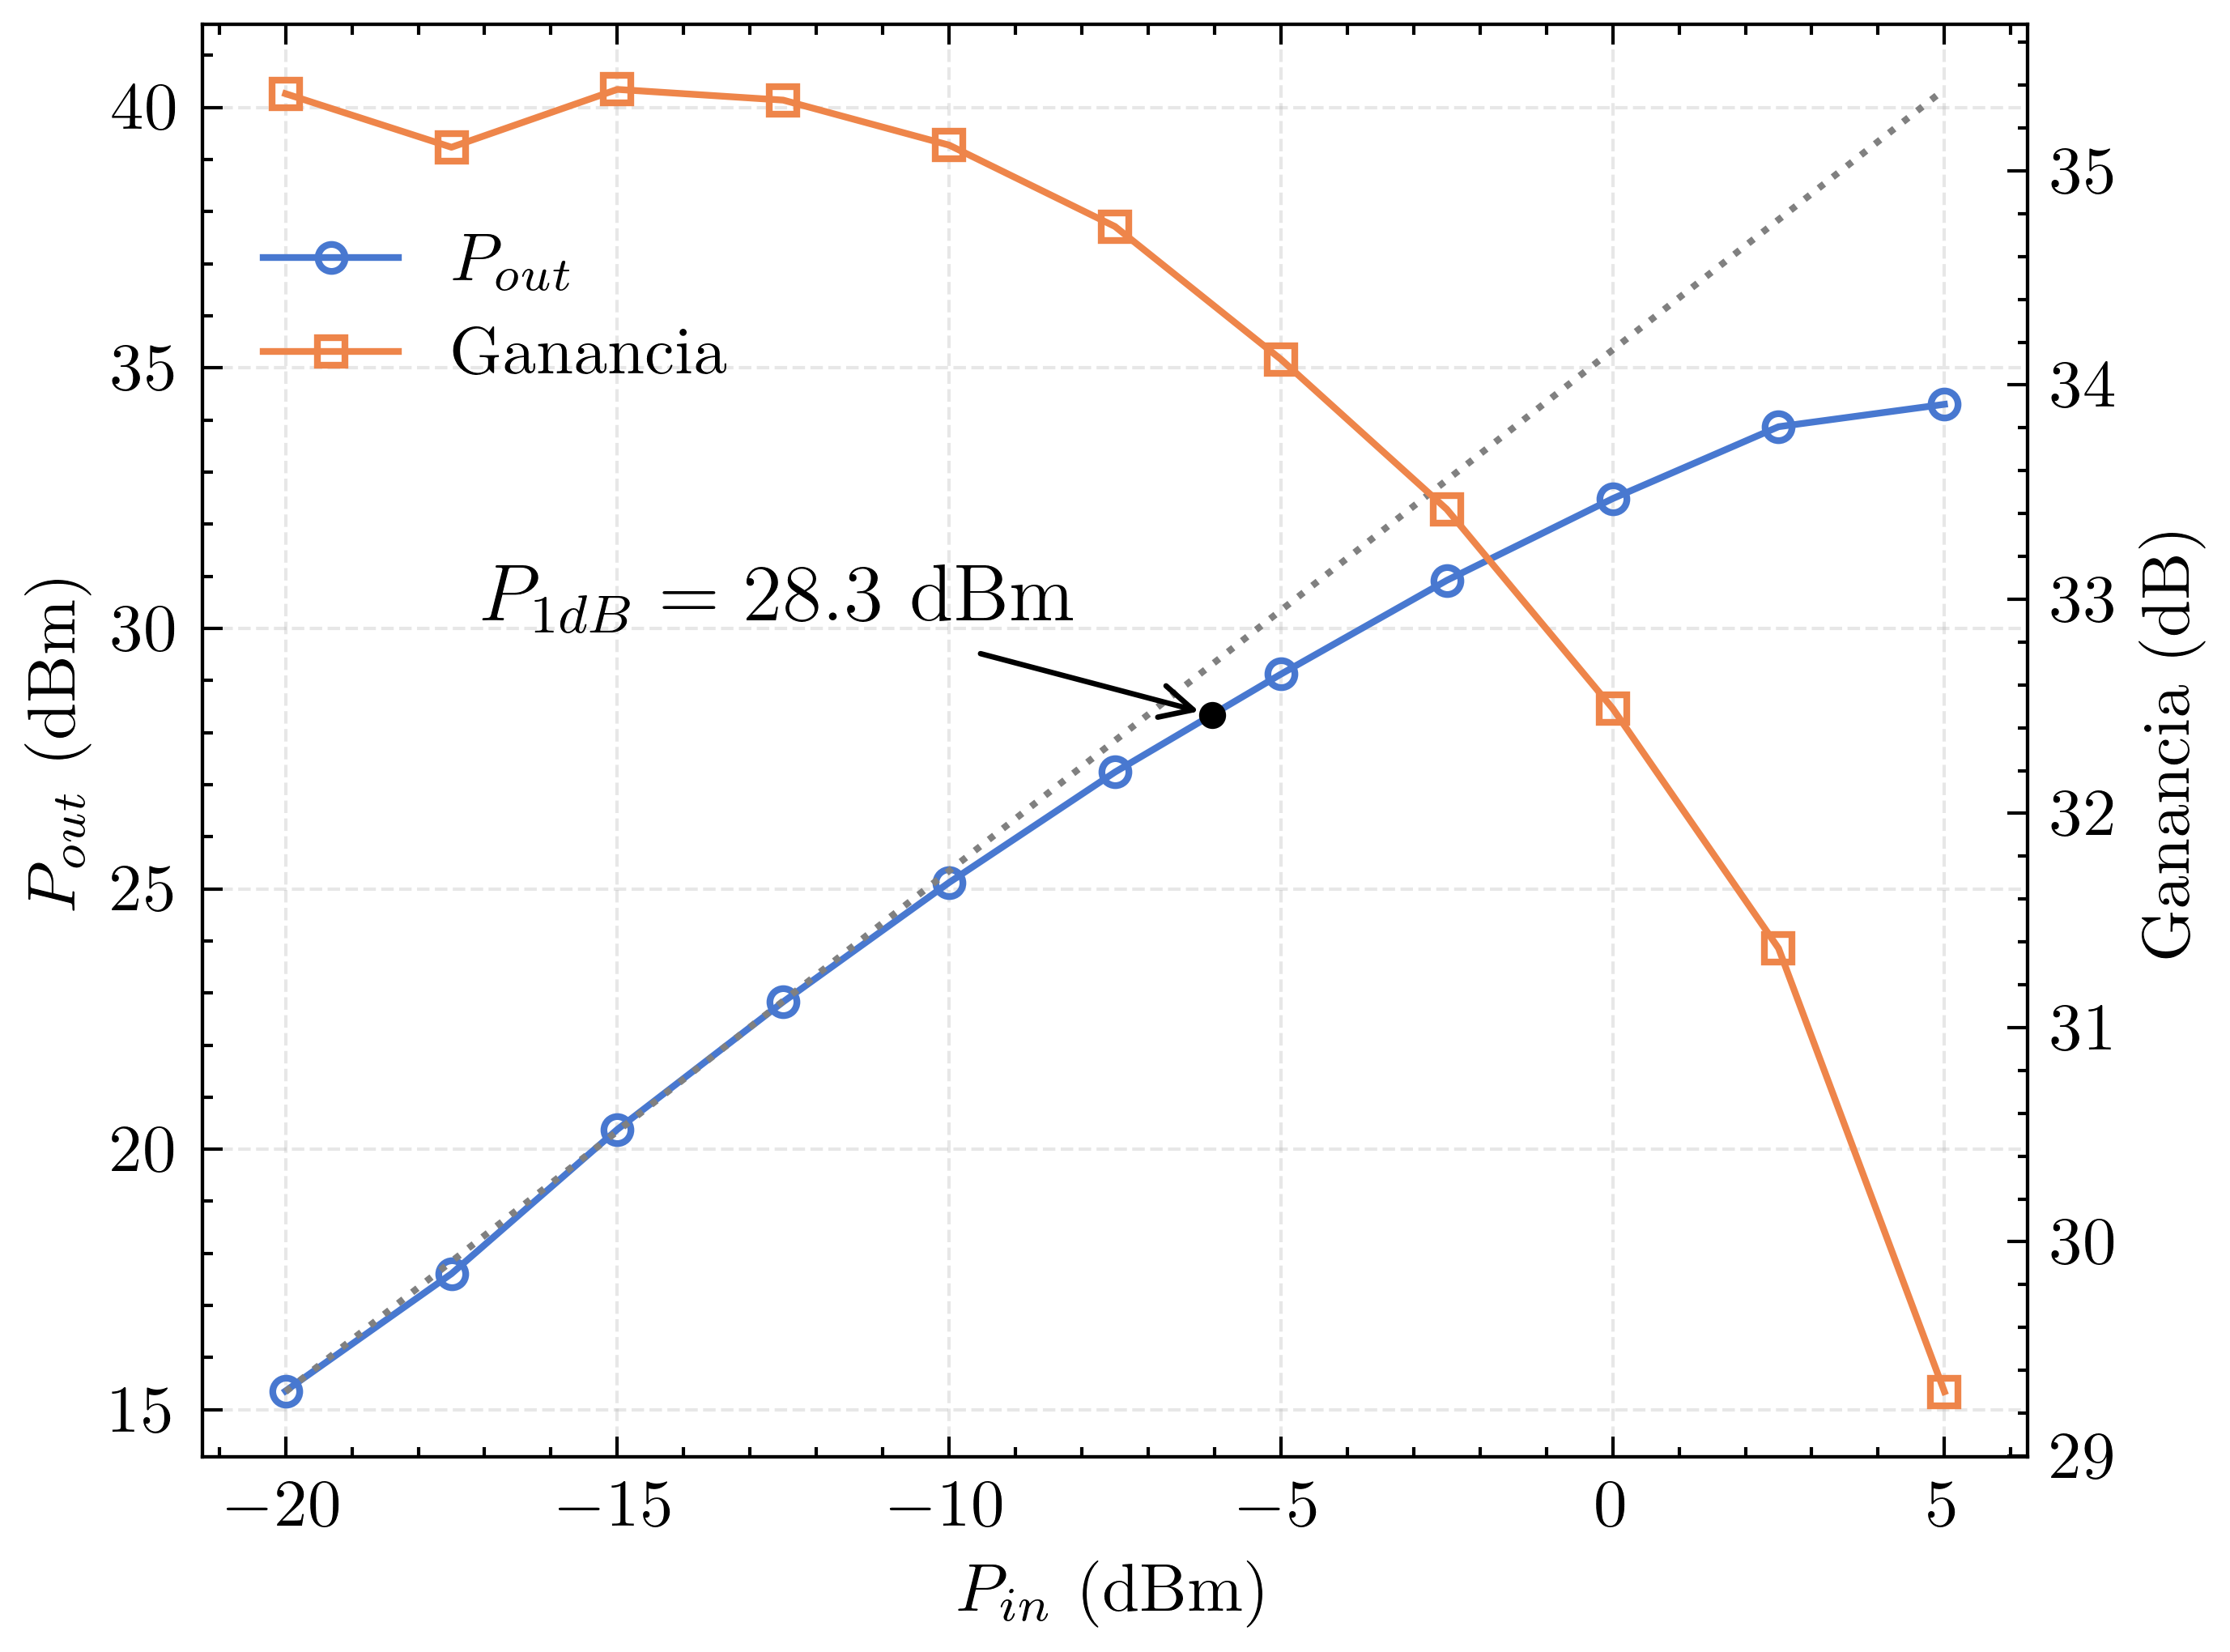
\includegraphics[width=0.8\linewidth]{Figures/08/pa_p1db_meas.png}
    \caption{Potencia de salida medida (azul) y ganancia (naranja) en función de la potencia de entrada para la cadena driver-DUT. La línea punteada gris representa la característica de transferencia lineal ideal obtenida de la extrapolación de ganancia de pequeña señal.}
    \label{fig:p1db}
\end{figure}

\begin{figure}[H]
    \centering
    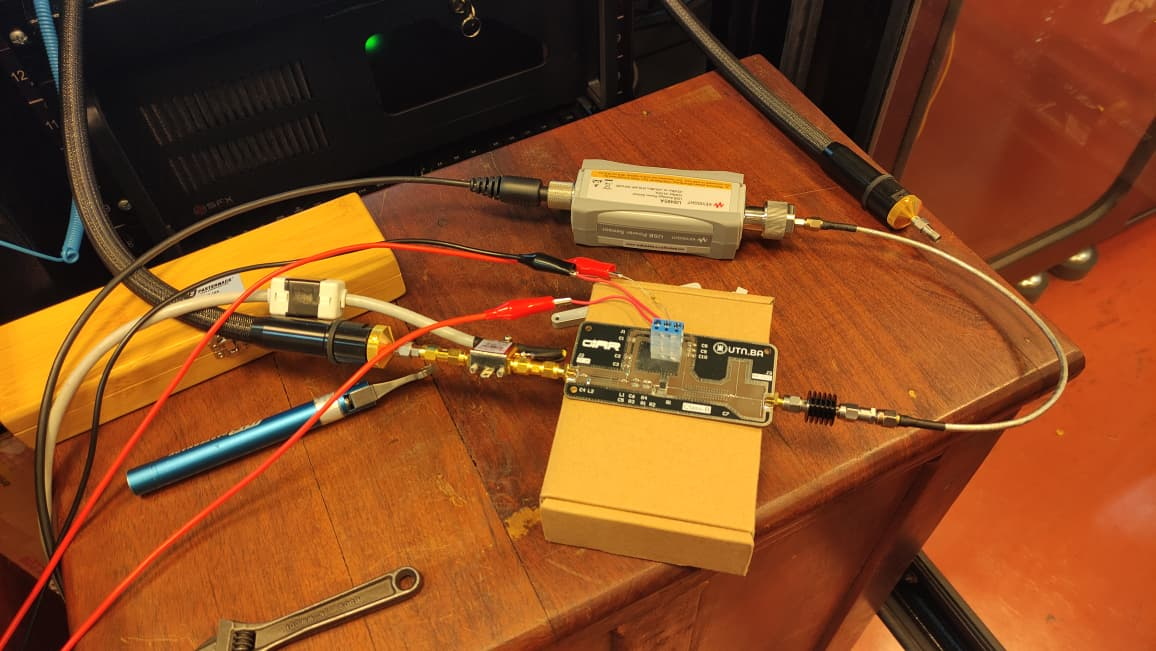
\includegraphics[width=\linewidth]{Figures/08/pa_setup_pout.jpg}
    \caption{Setup de medición empleado para la medición de la potencia de salida del amplificador de potencia en la CNEA.}
    \label{fig:setup_cnea_pout}
\end{figure}

% -----------------------------------------------------------------------------------------------%
\subsection{Ganancia, eficiencia de drain y ancho de banda}
\subsubsection{Ganancia}
La ganancia de pequeña señal del amplificador se extrajo a partir de la cadena de medición de potencia. La potencia de entrada y de salida en los terminales del amplificador se calcularon como

\begin{equation}
    P_{in,PA} = P_{in,sys} + G_{driver}
    \label{eq:pin_pa}
\end{equation}

\begin{equation}
    P_{out,PA} = P_{out,sys} + |A_{att}|
    \label{eq:pout_pa}
\end{equation}

donde $P_{in,sys}$ es la potencia de entrada del sistema, $G_{driver}$ es la ganancia de la etapa driver, $P_{out,sys}$ es la potencia de salida medida del sistema y $|A_{att}|$ es la atenuación total de la cadena de atenuadores, con todas las magnitudes expresadas en dBm y dB respectivamente. La ganancia se calculó entonces como

\begin{equation}
G = P_{out,PA} - P_{in,PA}
\label{eq:gain_calc}
\end{equation}

De esta manera se obtuvo una ganancia de pequeña señal de 13,26\,dB.

% -----------------------------------------------------------------------------------------------%
\subsubsection{Eficiencia de drain y PAE}
La eficiencia de drain ($\eta_D$) y la PAE se evaluaron a partir de la misma cadena de medición de potencia empleada para la extracción del P1dB, calculándose respectivamente como

\begin{equation}
    \eta_{D} = \frac{P_{out,PA}}{P_{DC}} \times 100\%
    \label{eq:drain_eff}
\end{equation}

\begin{equation}
    PAE = \frac{P_{out,PA} - P_{in,PA}}{P_{DC}} \times 100\%
    \label{eq:pae_calc}
\end{equation}

donde $P_{out,PA}$ y $P_{in,PA}$ son la potencia de salida y de entrada del amplificador obtenidas mediante las ecuaciones~\eqref{eq:pin_pa} y \eqref{eq:pout_pa}, y $P_{DC}$ es la potencia de continua entregada por la fuente de alimentación. La Figura~\ref{fig:pae_drain_eff} muestra ambas magnitudes en función de la potencia de salida entregada por el amplificador.

\begin{figure}[H]
    \centering
    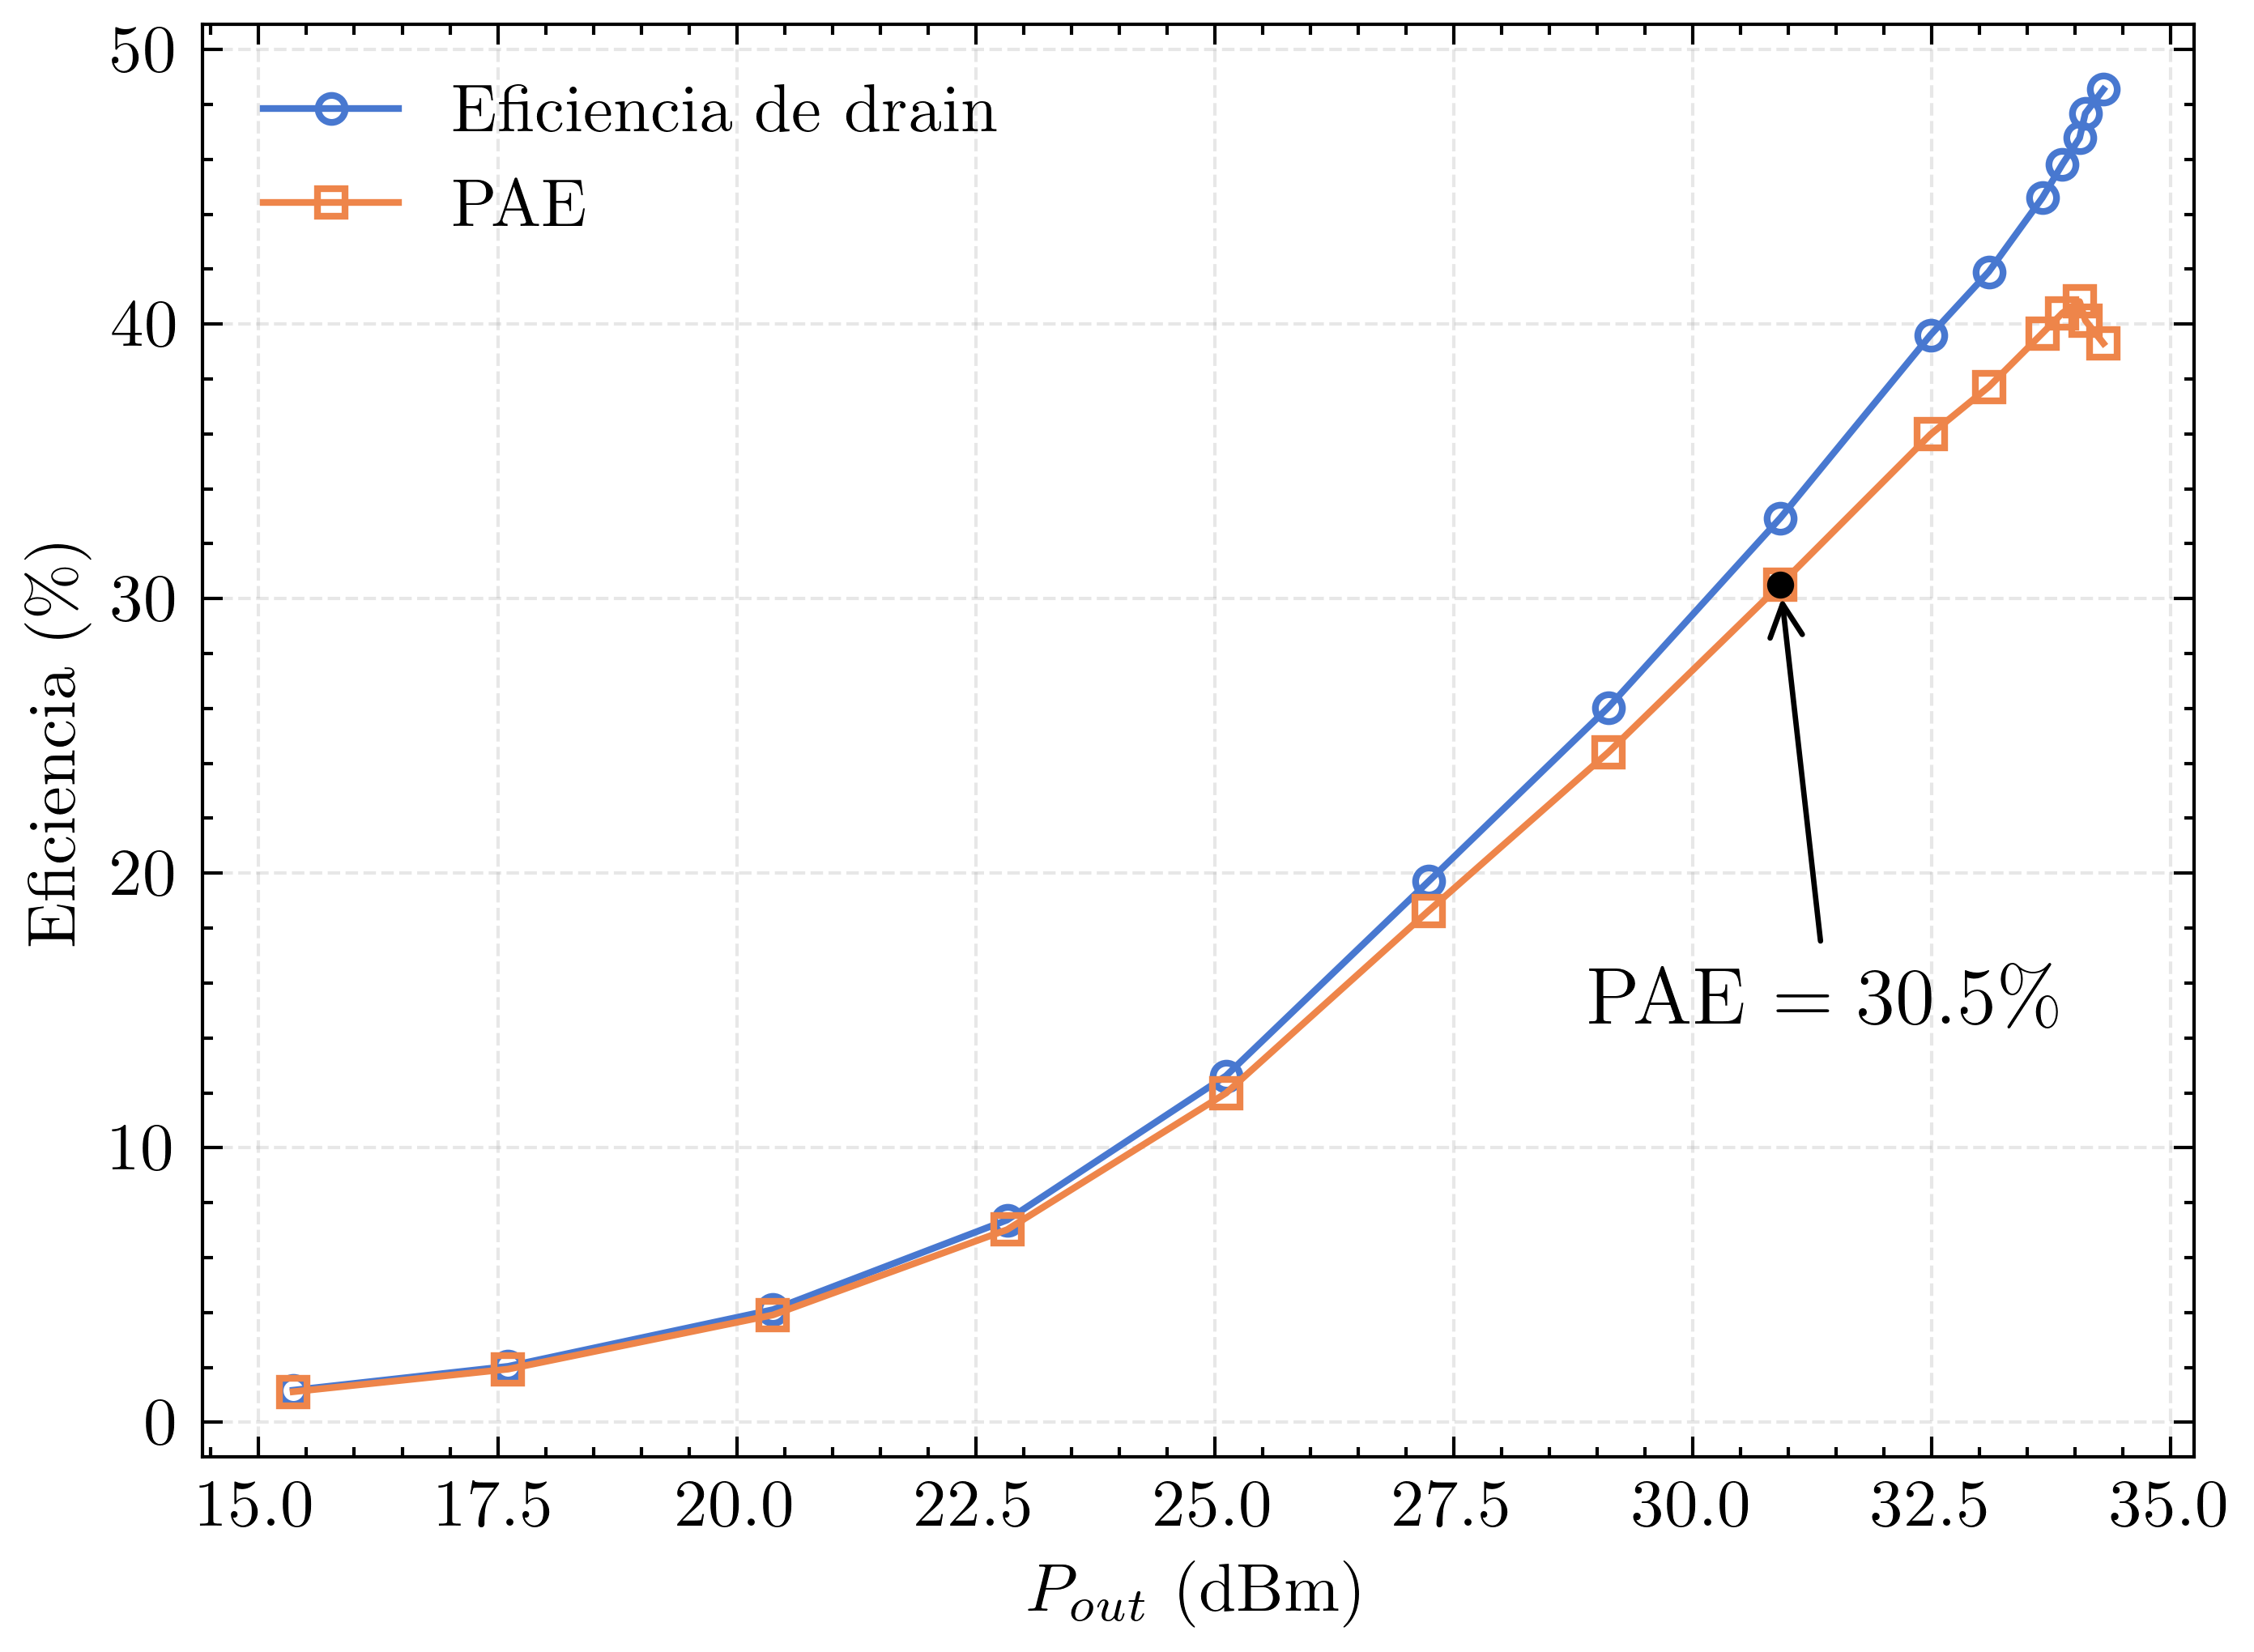
\includegraphics[width=0.8\linewidth]{Figures/08/pa_pae_drain_eff.png}
    \caption{Eficiencia de drain y PAE medidas en función de la potencia de salida del amplificador.}
    \label{fig:pae_drain_eff}
\end{figure}

Ambas magnitudes crecen con la potencia de salida, y la eficiencia de drain se mantiene siempre por encima de la PAE, tal como exige la relación entre ambas establecida en la ecuación~\eqref{eq:pae_definicion}. En el punto de medición más cercano al P1dB, correspondiente a una potencia de salida de 30,92\,dBm, se obtuvo una eficiencia de drain de 32,94\% y una PAE de 30,51\%.

% -----------------------------------------------------------------------------------------------%
\subsubsection{Ancho de banda}
El ancho de banda de operación se determinó a partir de la respuesta medida de $S_{11}$. Se identificaron los dos puntos de frecuencia en los cuales $S_{11}$ cruza el umbral de -10\,dB dentro de la región de interés, y el ancho de banda se definió como la diferencia entre ambos, método mediante el cual se obtuvo un valor de 70\,MHz para el ancho de banda.

% -----------------------------------------------------------------------------------------------%
\subsection{Distorsión armónica medida}
El segundo y el tercer armónico se midieron replicando el setup de la Figura~\ref{fig:setup_medicion_armonicos} en la UNSAM, ilustrado en la Figura~\ref{fig:setup_unsam_armonicos}, para una potencia de entrada barrida de 0 a 20\,dBm en pasos de 5\,dBm. 

\begin{figure}[H]
    \centering
    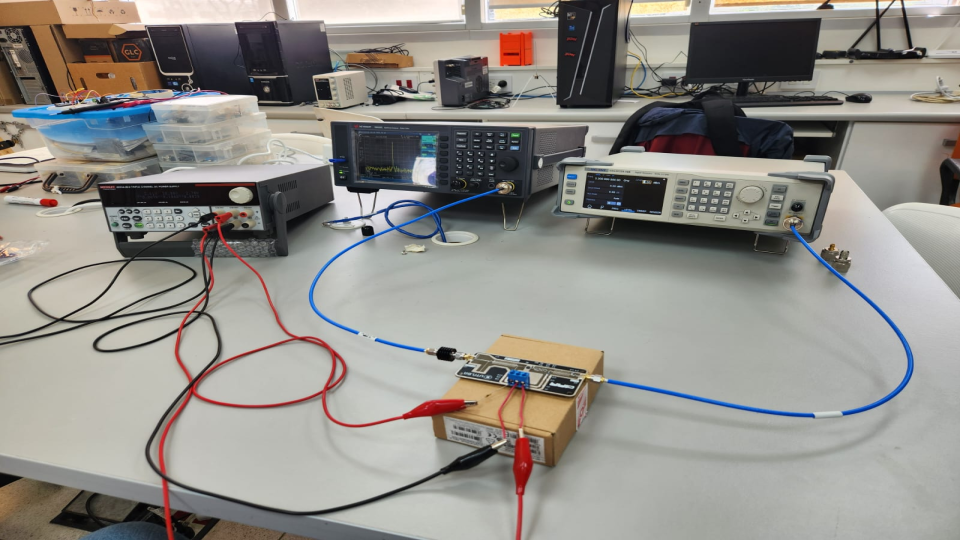
\includegraphics[width=\linewidth]{Figures/08/pa_setup_armonicos.png}
    \caption{Configuración de instrumentos utilizada para la medición de distorsión armónica del amplificador de potencia en la UNSAM.}
    \label{fig:setup_unsam_armonicos}
\end{figure}

El Cuadro~\ref{tab:pa_armonicos_medidos} resume la potencia medida de la componente fundamental, el segundo y el tercer armónico para cada nivel de excitación, mientras que la Figura~\ref{fig:pa_hb_harmonics} muestra los tonos correspondientes al caso de mayor potencia de entrada ($P_{in}=20$\,dBm), representando la condición no lineal de peor caso dentro del rango medido.

\begin{table}[H]
    \centering
    \caption{Potencia medida de la frecuencia fundamental, el segundo y el tercer armónico en función de la potencia de entrada.}
    \label{tab:pa_armonicos_medidos}
    \begin{tabular}{cccc}
        \hline\hline
        \textbf{$P_{in}$} & \textbf{Fundamental} & \textbf{Segundo Armónico} & \textbf{Tercer Armónico} \\
        \hline
        0~dBm  & $-8,53$~dBm  & $-54,57$~dBm & $-86,22$~dBm \\
        5~dBm  & $-3,07$~dBm  & $-42,04$~dBm & $-73,21$~dBm \\
        10~dBm & $2,06$~dBm   & $-32,25$~dBm & $-56,36$~dBm \\
        15~dBm & $6,42$~dBm   & $-23,93$~dBm & $-40,80$~dBm \\
        20~dBm & $10,11$~dBm  & $-16,63$~dBm & $-32,10$~dBm \\
        \hline\hline
    \end{tabular}
\end{table}

\begin{figure}[H]
    \centering
    \begin{subfigure}{0.48\linewidth}
        \centering
        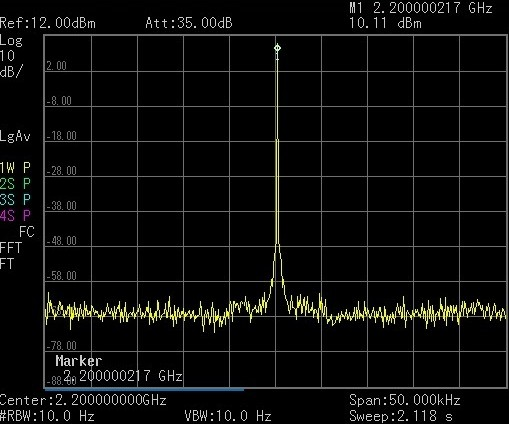
\includegraphics[width=\linewidth]{Figures/08/pa_hb_f1.jpg}
    \end{subfigure}
    \hfill
    \begin{subfigure}{0.48\linewidth}
        \centering
        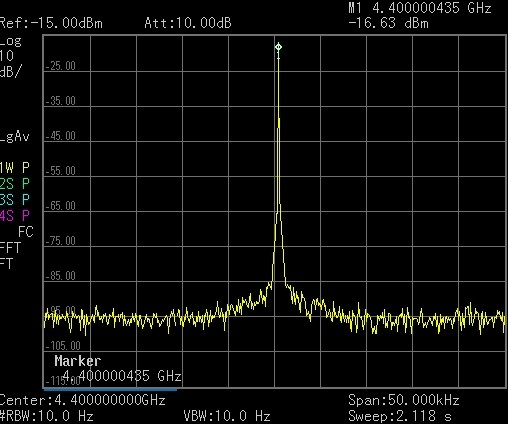
\includegraphics[width=\linewidth]{Figures/08/pa_hb_f2.jpg}
    \end{subfigure}
    \hfill
    \begin{subfigure}{0.48\linewidth}
        \centering
        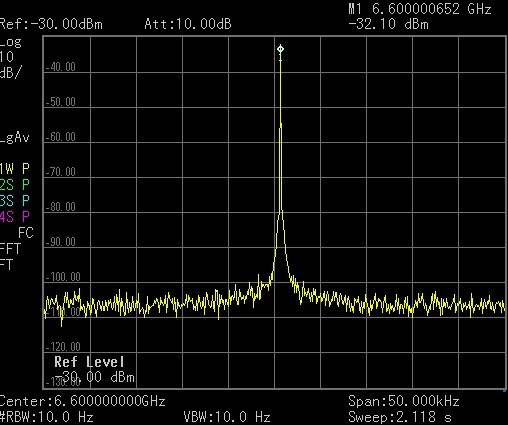
\includegraphics[width=\linewidth]{Figures/08/pa_hb_f3.jpg}
    \end{subfigure}
    \caption{Medición de potencia de tonos de frecuencia fundamental (arriba izq.), segundo armónico (arriba der.) y tercer armónico (abajo) para $P_{in}=20$\,dBm.}
    \label{fig:pa_hb_harmonics}
\end{figure}

Del Cuadro~\ref{tab:pa_armonicos_medidos} se desprende que el rechazo de ambos armónicos, definido como la diferencia entre la potencia de la componente fundamental y la del armónico correspondiente, se degrada de manera monótona a medida que aumenta la potencia de entrada, comportamiento consistente con el origen no lineal de la distorsión armónica. Para $P_{in}=20$\,dBm, aproximadamente en el punto de operación correspondiente al P1dB, el rechazo del segundo armónico fue de 26,74\,dBc y el rechazo del tercer armónico fue de 42,21\,dBc, representando el desempeño mínimo esperado en operación lineal por debajo de dicho punto. El contenido armónico medido difiere del simulado a nivel esquemático mostrado en la Figura~\ref{fig:pa_ads_armonicos}, lo cual se atribuye a un desplazamiento en frecuencia de la banda de rechazo del filtro de salida. Este efecto puede observarse en la respuesta de transmisión directa del amplificador ($S_{21}$), donde la banda de rechazo del filtro de salida aparece desplazada hacia frecuencias menores.

% -----------------------------------------------------------------------------------------------%
\subsection{OIP3 medido}
El OIP3 se determinó para la cadena conjunta del driver y el amplificador de potencia. La Figura~\ref{fig:oip3} muestra el OIP3 de la cadena para frecuencias entre DC y 5\,GHz. De manera análoga al caso del P1dB, la no linealidad del amplificador driver afecta el OIP3 de la cadena. Por este motivo, el valor de OIP3 correspondiente al dispositivo bajo prueba se obtuvo mediante la ecuación~\eqref{eq:oip3_cascada}

\begin{equation}
    OIP3_{Sys} = \left( \frac{1}{OIP3_{N-1} \cdot G_N} + \frac{1}{OIP3_N} \right)^{-1} \text{[mW]}
    \label{eq:oip3_cascada}
\end{equation}

Se obtuvo un OIP3 de 39,83\,dBm. Este valor resulta consistente con la relación empírica entre el P1dB y el OIP3 presentada en la ecuación~\eqref{eq:oip3_p1db}, dado que la diferencia de 9,53\,dB respecto de los 30,3\,dBm de P1dB medidos se aproxima al factor de 10\,dB allí indicado.

\begin{figure}[H]
    \centering
    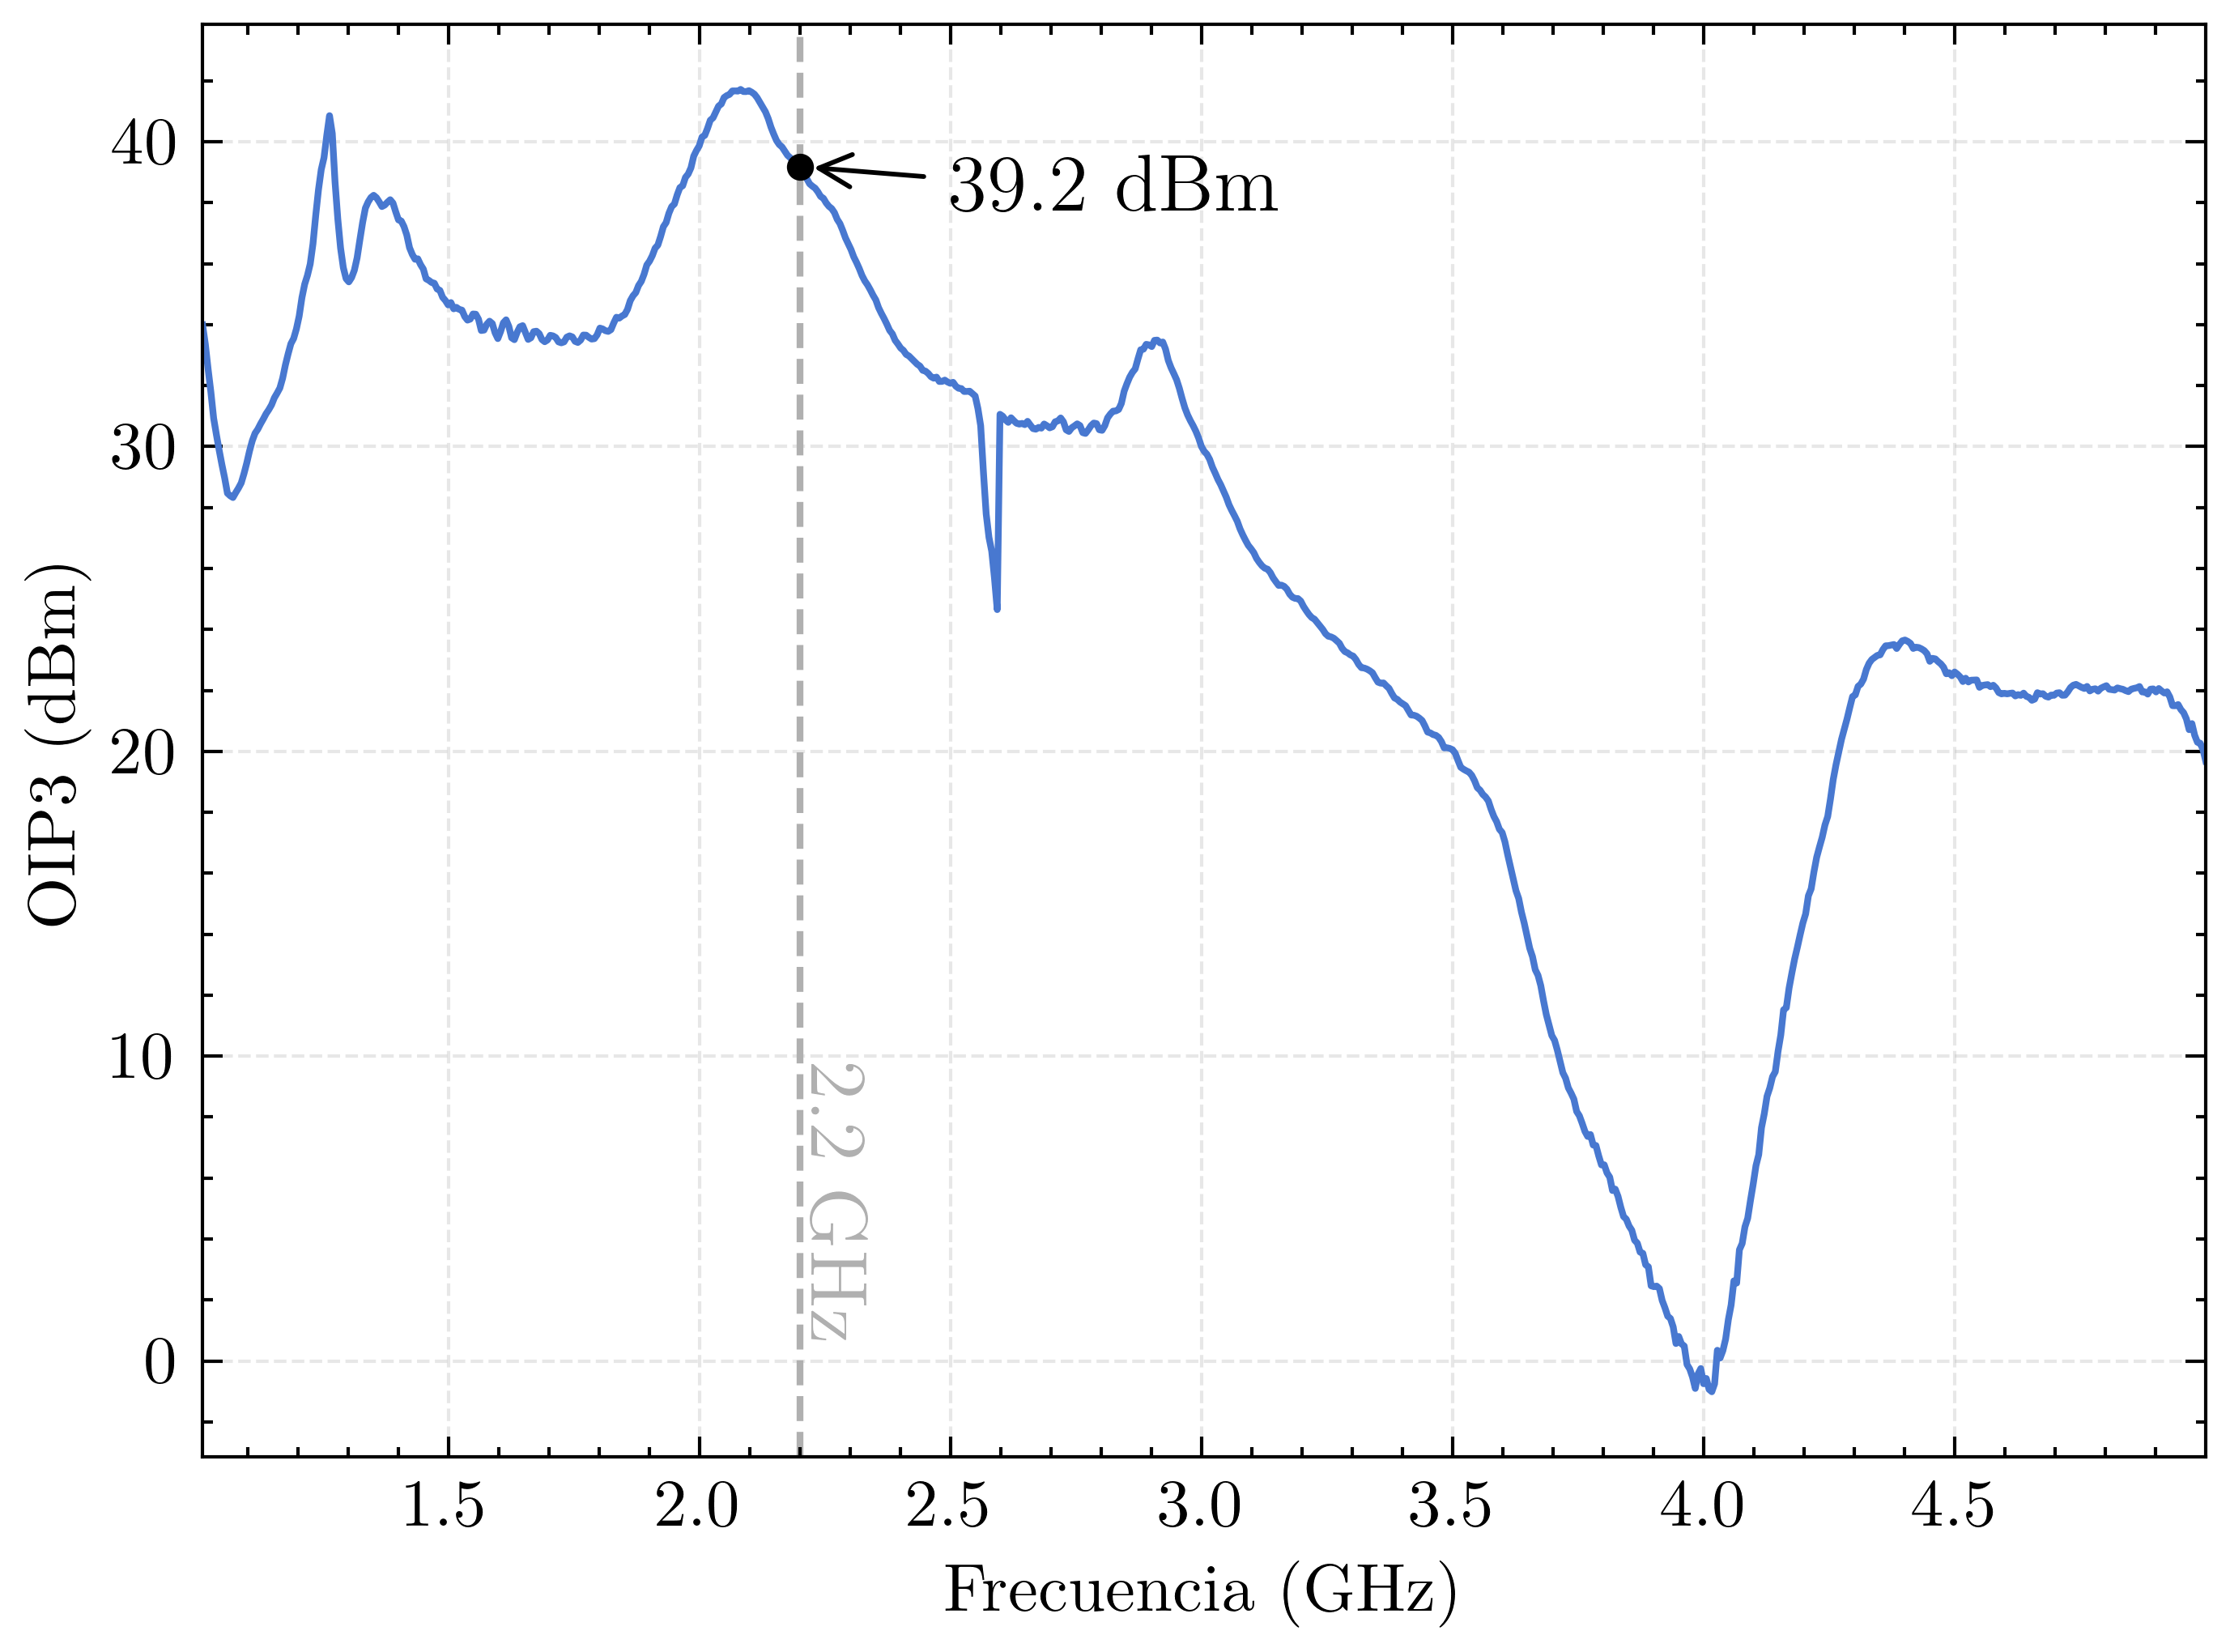
\includegraphics[width=0.8\linewidth]{Figures/08/pa_oip3_meas.png}
    \caption{Barrido en frecuencia del punto de intercepción de tercer orden a la salida (OIP3) medido para la cadena driver-DUT.}
    \label{fig:oip3}
\end{figure}

% -----------------------------------------------------------------------------------------------%
\subsection{Resumen de resultados}
El Cuadro~\ref{tab:resumen_resultados} presenta una vista consolidada de los resultados de caracterización descritos a lo largo de esta sección.

\begin{table}[H]
    \centering
    \caption{Resumen de Desempeño Medido del Amplificador de Potencia RF}
    \label{tab:resumen_resultados}
    \begin{tabular}{lc}
        \hline\hline
        \textbf{Parámetro} & \textbf{Valor} \\
        \hline
        Frecuencia Central & 2,11\,GHz \\
        \hline
        Ancho de Banda (BW) & 70\,MHz \\
        \hline
        Punto de Compresión de 1\,dB (P1dB) & 30,30\,dBm \\
        \hline
        Intercepción de Tercer Orden (OIP3) & 39,83\,dBm \\
        \hline
        Ganancia de Pequeña Señal & 13,26\,dB \\
        \hline
        Eficiencia de Drain & 32,94\% @ $P_{out} = 30{,}92\,$ dBm \\
        \hline
        PAE & 30,51\% @ $P_{out} = 30{,}92\,$ dBm \\
        \hline\hline
    \end{tabular}
\end{table}

Comparando estos resultados contra los objetivos de diseño establecidos en el Cuadro~\ref{tab:objetivos_diseno}, el amplificador fabricado satisface los requisitos mandatorios de ancho de banda, potencia de salida y OIP3. El ancho de banda medido duplica el mínimo exigido, la potencia de salida evaluada en las proximidades del P1dB (aprox. 1,24\,W) supera el objetivo de 1\,W, y el OIP3 medido de 39,83\,dBm excede el mínimo de 35\,dBm. La frecuencia central, en cambio, no cumple con el objetivo de diseño de 2,2\,GHz, dado que el corrimiento de 90\,MHz identificado en la Sección~\ref{sec:resultados_pa} ubica a la frecuencia objetivo por fuera del ancho de banda de operación medido, cuyo límite superior se encuentra a 2,145\,GHz. En cuanto al objetivo de PAE, el valor obtenido en las proximidades del P1dB se ubica por debajo del mínimo especificado, según se desprende de la Figura~\ref{fig:pae_drain_eff}. No obstante, dicha figura muestra que la PAE continúa creciendo más allá del P1dB, superando el 35\% objetivo a partir de una potencia de salida de aproximadamente 32,5\,dBm, aunque a costa de operar el amplificador en una región de compresión más profunda, con la consiguiente penalización sobre la linealidad de la señal amplificada.

Al comparar estos valores medidos con los obtenidos mediante simulación a nivel esquemático en el Cuadro~\ref{tab:pa_valores_importantes_ads}, es necesario considerar que ambos conjuntos de valores fueron evaluados en distintas condiciones de operación. La simulación se realizó para una potencia de entrada fija de 20\,dBm, mientras que los valores de gran señal medidos corresponden al punto de compresión de 1\,dB del dispositivo, ubicado a un nivel de excitación distinto. Con esta salvedad, la potencia de salida simulada de 36,157\,dBm a 20\,dBm de entrada resulta consistente con una curva de transferencia que satura en las proximidades de dicho valor, en tanto que la ganancia, la eficiencia de drain y la PAE simuladas exceden a las medidas, diferencia que resulta esperable dado el corrimiento de la frecuencia central y la resonancia parásita identificados en los parámetros de dispersión, ninguno de los cuales fue contemplado en el modelo esquemático original.

En conjunto, los resultados obtenidos validan la metodología de diseño empleada, al tiempo que identifican dos aspectos concretos de mejora para futuras iteraciones del circuito: la incorporación de la inductancia equivalente serie de los componentes discretos de la red de estabilidad desde las primeras etapas de simulación, en lugar de ser una corrección posterior a la medición, y un modelado más detallado de los efectos parásitos del layout físico y del empaquetado de los componentes, con el fin de anticipar la resonancia fuera de banda observada experimentalmente y reducir el desplazamiento de la banda de rechazo del filtro de salida identificado en la caracterización de distorsión armónica.